The understanding of spontaneous symmetry breaking and cosmological phase transitions has led us to think about the possible existence of topological defects formed in the early universe. Topological defects are related to spontaneous symmetry breaking since they give rise to a non-trivial vacuum manifold. For instance, the spontaneous symmetry breaking of a global or local U(1) symmetry can lead to 1-dimensional topological excitations known as vortices, and when these vortices form lines in the 3-dimensional space they are called vortex strings. 
 
\section{The creation of cosmic strings in the early universe} 
Let us illustrate the formation of cosmic strings through the Kibble mech\-an\-ism. Suppose we have a field theory, with a complex order parameter scalar field $\phi$, with a $\text{U}(1)$ symmetry and with a potential suitable for spontaneous symmetry breaking to happen. Due to high temperatures in the early universe, the field con\-fig\-u\-ra\-tions initially remained in a state of unbroken symmetry. When the temperature decreased as the universe expanded, spontaneous symmetry breaking occurred and different regions of the universe remained isolated from each other. In each isolated region, the field acquired a different vacuum expectation value. The patches grew and became casually connected giving rise to topological defects. If these uncorrelated regions formed a loop around some line such that the field values along the loop completed $n$ turns, the topological defect is in fact a \textit{cosmic string} with a winding number of $n$, see Figure \ref{fig:higgspotential}. %and if the  In this example, since we are dealing with a U(1) symmetry in a 3-dimensional space, the topological defects are in fact strings which we call \textit{cosmic strings}.
\begin{figure}
	\centering
	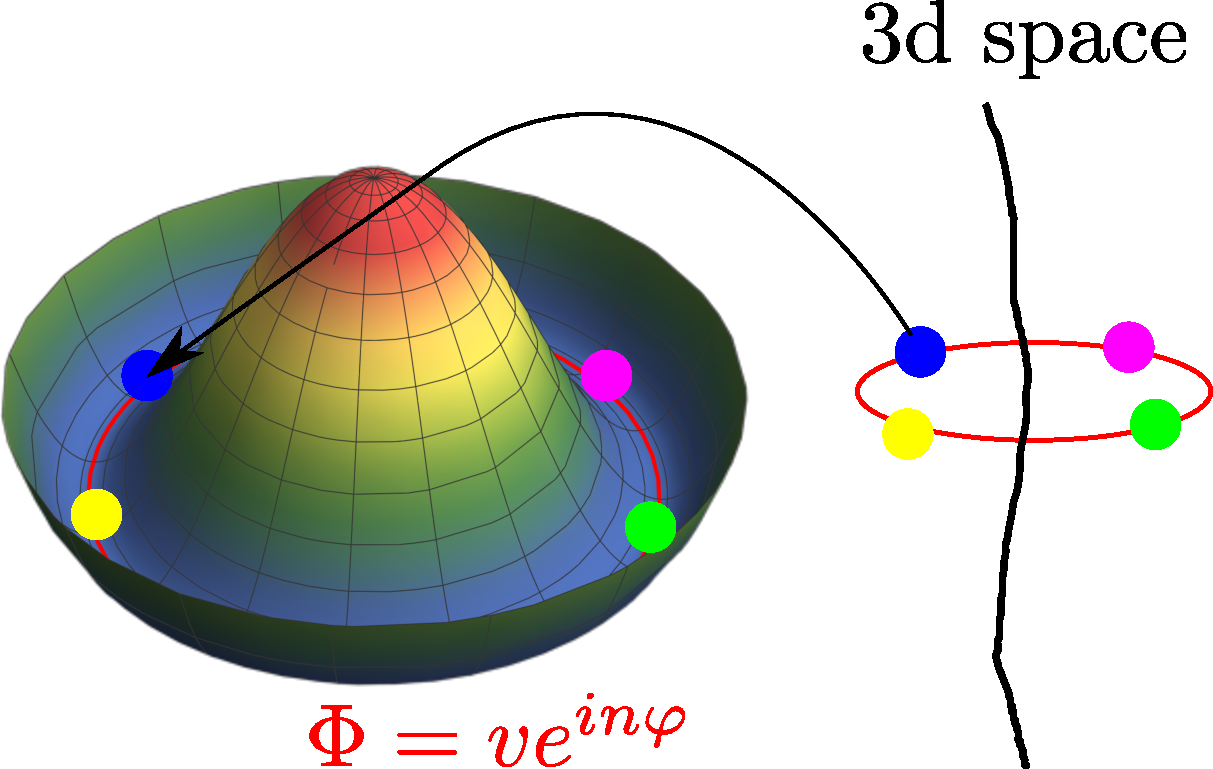
\includegraphics[scale=0.65]{./figures/higgspot.pdf}
	\caption{The formation of a cosmic string. When different uncorrelated points in the universe became casually connected, the different vacuum-values the field took in these points gave rise to topological defects.}
	\label{fig:higgspotential}
\end{figure} 
%\begin{figure}
%	\centering
%	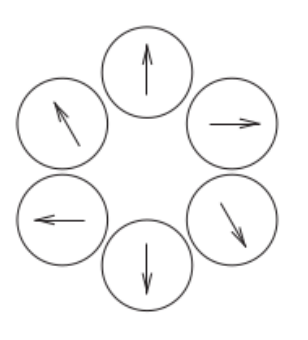
\includegraphics[scale=0.5]{./figures/vortex.png}
%	\caption{Vortex.}
%	\label{fig:vortex}
%\end{figure} 
\section{Global cosmic strings}\label{sec:global}
We consider the simplest model where string-like solutions appear: a scalar field $\phi(x)\in\mathbb{C}$ with a global U(1) symmetry and a Lagrangian density given by
\begin{equation}
	\mathcal{L} = \frac{1}{2}\partial^{\mu} \phi^* \partial_{\mu} \phi  \underbrace{-\frac{m^2}{2} |\phi|^2 - \frac{\lambda}{4}|\phi|^4-\frac{\lambda}{4}v^4}_{-V(\phi)} ,
\end{equation}
where $m^2$ and $\lambda$ refer to the renormalized values.
We require $\lambda>0$, in order for the potential to be bounded from below. We find the potential minima by differentiating with respect to $|\phi|$
\begin{equation}
	\left.\frac{dV}{d|\phi|}\right|_{\phi_0\in\mathcal{M}} = m^2 |\phi_0|+\lambda |\phi_0|^3 = 0 \Rightarrow \begin{cases} |\phi_0|^2 = -\frac{m^2}{\lambda} \text{ only if } m^2<0 \\ 
	|\phi_0| = 0 \text{ if } m^2 \geq 0.
	\end{cases}
\end{equation}
If $m^2 < 0$, it leads to the spontaneous symmetry breaking of the U(1) symmetry. Then the vacuum expectation value is
\begin{equation}
	|\phi_0| = v \equiv \sqrt{\frac{-m^2}{\lambda}}.
\end{equation}
We consider a cylindrically symmetric, static field configuration
\begin{equation}
	\phi = \phi(r,\varphi,z) = \phi (r,\varphi) .
\end{equation}
At $r \to \infty$, the field configuration $\phi$ must take its vacuum expectation value $v$, $\lim\limits_{r\to\infty}|\phi(r,\varphi)| = v$. But the complex phase can be any differentiable function of $\varphi$. Therefore our ansatz takes the form
\begin{equation}
	\lim_{r\to\infty}\phi(r,\varphi) = \phi^{\infty}(\varphi) = v e^{i\chi(\varphi)} . 
\end{equation}
The function $\phi^{\infty}$ maps $S^1 \to \mathcal{M} = S^1= $ U$(1)$. Since $\pi_1[S^1] = \mathbb{Z}$, the model allows for vortex solutions and there is a winding number $n\in\mathbb{Z}$. Global strings are configurations with $n\neq 0$, which are topologically stable, i.e., stable under continuous deformations. We assume $\chi(\varphi) = n\varphi$ with $n\neq 0$. Our ansatz becomes
\begin{equation}
	\phi(r,\varphi) = f(r)e^{in\varphi},
\end{equation}
where 
\begin{equation}
	\lim_{r\to\infty}f(r) = v,\ \ \ f(0) = 0.
	\label{eq:limits} 
\end{equation}
The latter relation is due to the fact that the field $\phi$ must be single valued. The field equation of motion reads
\begin{equation}
	\partial^{\mu}\partial_{\mu}\phi = -m^2\phi -\lambda |\phi|^2 \phi ,
\end{equation}
using cylindrical coordinates
\begin{eqnarray}
	\frac{1}{r} \partial_{r} (r\partial_{r}\phi) + \frac{n^2}{r^2}\partial_{\varphi} \phi = m^2 \phi + \lambda |\phi|^2 \phi \nonumber \\
	\frac{1}{r} \partial_{r} (r f')e^{i\varphi} - \frac{n^2}{r^2} f e^{i\varphi} = m^2 fe^{i\varphi} + \lambda f^3 e^{i\varphi} \nonumber \\
	\label{eq:global_str}
	f'' + \frac{1}{r}f'- \frac{n^2}{r^2} f = m^2 f+ \lambda f^3.
\end{eqnarray}
We arrive at a non-linear second order differential equation. We can obtain its asymptotic behavior at large $r$ and near zero, with the constraints of eq. \eqref{eq:limits}.
If $r\approx 0$, we only keep the linear powers of $f$, so eq. \eqref{eq:global_str} simplifies to
\begin{equation}
	f'' + \frac{1}{r}f'- \frac{n^2}{r^2} f -m^2 f\approx  0.
\end{equation}
Inserting $m^2 = -v^2\lambda$, we obtain
\begin{equation}
	f'' + \frac{1}{r}f'- \frac{n^2}{r^2} f + v^2\lambda f\approx  0.
\end{equation}
If we substitute $u=\sqrt{v^2\lambda}r$, then $f(r) = \tilde{f}(u)$ and we obtain Bessel's equation for $\tilde f$
\begin{equation}
	\frac{d^2\tilde f}{du^2} + \frac{1}{u}\frac{d\tilde f}{du}+\left(1- \frac{n^2}{u^2}\right) \tilde f\approx  0\, ,
\end{equation}
with the solution
\begin{equation}
	\tilde f(u) \approx  f_0 J_{|n|}(u) +  \tilde f_1 Y_{|n|}(u),
\end{equation}
where $J_{|n|}$ and $Y_{|n|}$ are the Bessel functions of the first and second kind of order $n$, respectively, and $f_0$ and $\tilde f_1$ are real constants. We set $\tilde f_1=0$ since $Y_{|n|}$ diverges at zero.
Then the solution is
\begin{equation}
	\tilde f(u) \approx f_0 J_{|n|}(u) = f_0 J_{|n|}(\sqrt{v^2\lambda}r)\, .
\end{equation}
Therefore
\begin{equation}
	f(r) \approx f_0 J_{|n|}(\sqrt{v^2 \lambda}r) = f_0\sum_{m=0}^{\infty}\frac{(-1)^m}{m!\Gamma(m+|n|+1)}\left(\frac{\sqrt{v^2 \lambda}r}{2}\right)^{2m+|n|}
\end{equation}
and to order $n$ in $r$ we have
\begin{equation}
	f(r) \approx f_0 \frac{1}{|n|!}\left(\frac{\sqrt{v^2 \lambda}r}{2}\right)^{|n|}.
	\label{eq:solr0}
\end{equation}
%The absolute value of $|n|$ comes from the fact that when $n\to-n<0$, $J_{-n}=(-1)^nJ_n$.
%Making the ansatz $f(r) = f_0 r^l$ we arrive to $l = \pm n$. So
%\begin{equation}
%	f(r) \approx f_0 r^n + \tilde f_0 r^{-n}
%\end{equation}
%where $f_0$ and $\tilde f_0$ are real constants. Since $f(0)=0$, we need a solution that does not explode at $r = 0$. If $n>0$ we take $f_0 r^n$ and if $n<0$ we take $\tilde f_0 r^{-n}$. Combining these two results we get
%\begin{equation}
%	\label{eq:phi_r0}
%	f(r) \approx f_0 r^{|n|} \text{ when } r\approx 0 \, .
%\end{equation}
At $r\to\infty$, $f(r)$ approaches its vacuum expectation value $v$. If we write in this limit $f(r) = v + \delta f(r)$, and ignoring O$(\delta f^2)$ terms, eq.\ \eqref{eq:global_str} turns into an equation for $\delta f$
\begin{equation}
	 \delta f'' +\frac{1}{r}\delta f'- \frac{|n|^2}{r^2}\delta f -2v^2\lambda\delta f \approx 0\, .
\end{equation}
When we perform the change of  variable $u=\sqrt{2\lambda}vr$ the equation above turns into the modified Bessel equation
\begin{equation}
\frac{d^2 }{du^2}\delta f + \frac{1}{u} \frac{d}{du}\delta f - \left(1+\frac{|n|^2}{u^2} \right)\delta f \approx 0\,.
\end{equation}
This equation has the solution
\begin{equation}
	\delta f \approx \tilde f_0I_{|n|}(u) + f_1 K_{|n|}(u) = \tilde f_0 I_{|n|}(\sqrt{2\lambda}vr) + f_1 K_{|n|}(\sqrt{2\lambda}vr)
\end{equation}
where $I_{|n|}$ and $K_{|n|}$ are the modified Bessel function of the first and second kind, respectively, and $\tilde f_0$ and $f_1$ are real constants. Since $I_{|n|}$ diverges when $r\to \infty$, we set $\tilde f_0=0$. Hence, the solution for $f$ at $r\to\infty$ takes the form
\begin{equation}
	f(r) \approx v+f_1 K_{|n|}(\sqrt{2\lambda}vr)\, .
\end{equation}

%If we write in this limit $f = v - \delta f$ we get
%\begin{equation}
%	-\frac{n^2}{r^2} \approx m^2 + \lambda (v-\delta f)^2 = m^2 + \lambda v^2 -2\lambda v \delta f + O(\delta f^2).
%\end{equation}
%Thus
%\begin{equation}
%	\delta f \approx \frac{n^2}{2\lambda v r^2}.
%\end{equation}
In summary
\begin{equation}
	\label{eq:asymptotic_global}
	f(r) \approx \begin{cases}
		\displaystyle f_0 \frac{1}{n!}\left(\frac{\sqrt{\lambda}vr}{2}\right)^{|n|}& r \ll 1 \\
	\displaystyle v+f_1\sqrt{\frac{\pi}{2\sqrt{2\lambda}v}}r^{-1/2}e^{-\sqrt{2\lambda}vr} & r \gg 1\, ,
				\end{cases}
\end{equation}
where in the second line we used the asymptotic behavior of $K_n$. %If we consider $n<0$, we find similar behaviors of the solution at the limits. we may write the winding number in the solutions as an absolute value $n$. 
\subsection{Energy density}
The expression for the energy density reads
\begin{equation}
	\label{eq:energy_density}
	\varepsilon(r) = \cancelto{0}{\frac{1}{2}|\partial_t \phi|^2} +\frac{1}{2}|\partial_r \phi|^2 + \frac{1}{2}\left|\frac{1}{r}\partial_{\varphi} \phi \right|^2 +\frac{1}{2}|\partial_z \phi|^2   + V(\phi).
\end{equation}
The first term is zero since $\phi$ is a static configuration.
Because of the angular derivative term, the energy density is of O$(1/r^2)$ at large $r$. Thus the energy per unit length along the $z$ direction, inside a cylinder of external radius $R\to \infty$ and internal radius $\delta\to 0$, diverges logarithmically, that is
\begin{equation}
	\frac{E}{z} \sim \int_{0}^{2\pi}d\varphi \int_{\delta}^{R}  dr  \ r\frac{1}{r^2} \propto \lim_{R\to\infty, \delta\to 0}\log \frac{R}{\delta} .
\end{equation}
%We can interpret this divergence due to the interaction of the string with the Nambu-Goldstone Boson given by the imaginary part of the field.
%The main implication of this result is that global strings have infinite length. Otherwise, there will be an infinite energy gap. 
Figure \ref{fig:global_str} shows the profile of a global string type solution of eq.\ \eqref{eq:global_str}, obtained with numerical methods, which is in agreement with the asymptotic behavior specified in eq.\ \eqref{eq:asymptotic_global}. 

\begin{figure}
	\centering
		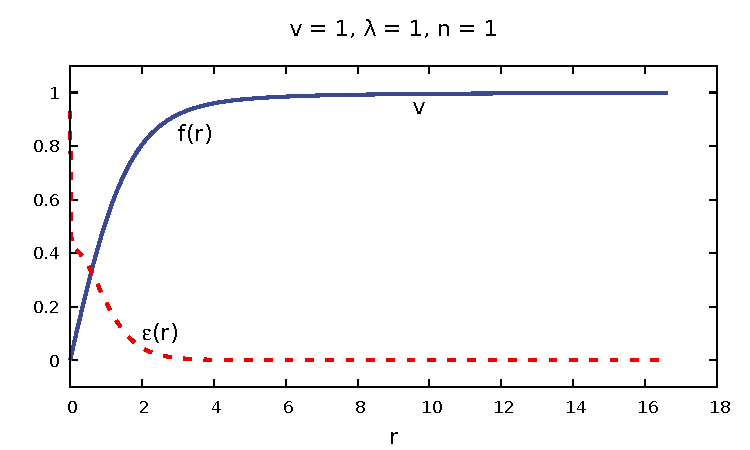
\includegraphics[scale=1]{./figures/global_str.pdf}
	\caption{Radial profile of a global string and its energy density.}
	\label{fig:global_str}
\end{figure}

\section{Local cosmic strings}\label{sec:local}
In order to promote U(1) to a local symmetry, we need to add a gauge field $A_{\mu}$. So the Lagrangian becomes
\begin{equation}
	\mathcal{L} = \frac{1}{2}(D^{\mu} \phi)^* D_{\mu} \phi - \frac{m^2}{2} |\phi|^2 - \frac{\lambda}{4}|\phi|^4 - \frac{\lambda}{4}v^4 - \frac{1}{4}F^{\mu\nu}F_{\mu\nu},
\end{equation}
where $D_{\mu}\phi = (\partial_{\mu} + ihA_{\mu})\phi$ is the covariant derivative, $h$ is a gauge coupling and $F_{\mu\nu} = \partial_{\mu}A_{\nu} - \partial_{\nu}A_{\mu}$ is the field strength tensor. Now, the equations of motion are
\begin{eqnarray}
	D^{\mu}D_{\mu} \phi & = & -m^2 \phi - \lambda|\phi|^2\phi, \\
	D^{\mu}F_{\mu\nu} & = & -\frac{ih}{2}\left[(D_\nu \phi)^* \phi - \phi^* D_{\nu}\phi\right].
\end{eqnarray}
We write the generic, static, cylindrical ansatz as
\begin{equation}
	\phi(r,\varphi) = f(r)e^{in\varphi}, \ \ \ \vec{A}(r,\varphi) = \frac{a(r)}{r}\hat{\varphi},
\end{equation}
where we have chosen the radial gauge where $A_r = 0$. For the functions to be continuous at the origin $f(0) = 0$ and $a(0)=0$.
Using the ansatzë for the functions the equations for $f$ and $a$ take the form
\begin{eqnarray}
	 \label{eq:local_f}
	f'' + \frac{1}{r} f' - \frac{1}{r^2}\left(n+ha\right)^2f- m^2 f- \lambda f^3= 0, \\
	\label{eq:local_a}
	a'' -\frac{1}{r}a'-h(n+ha)f^2= 0.
\end{eqnarray}
From eq.\ \eqref{eq:local_a} we obtain the asymptotic behavior of the function $a(r)$. At large $r$ we expect the function to be constant, this is only achieved if the term in parenthesis is zero, which implies $\lim_{r\to\infty}a(r) = -n/h$.

Again, the system is not analytically solvable, but we can derive its asymptotic behavior.

When $r \to 0$, eq.\ \eqref{eq:local_f} is approximately (assuming $f(r) = $ O$(r)$)
\begin{equation}
	 f'' + \frac{1}{r} f'  -\frac{n^2}{r^2}f -m^2 f\approx 0, 
\end{equation}
so again as in eq.\ \eqref{eq:solr0} the approximate solution is 
\begin{equation}
	f(r) \approx f_0 \frac{1}{|n|!}\left(\frac{\sqrt{v^2 \lambda}r}{2}\right)^{|n|} .
\end{equation}
In this limit, eq.\ \eqref{eq:local_a} takes the form
\begin{equation}
	a'' - \frac{1}{r}a' \approx 0
\end{equation}
and its solution is
\begin{equation}
	a(r) \approx \frac{a_0}{2}r^2,
\end{equation}
where $a_0$ is a constant.

In order to study the limit $r\to\infty$, we use $f = v + \delta f$ and $a = -\frac{n}{h} + \delta a$, and ignore quadratic terms in $\delta f$ and $\delta a$. Then eq.\ \eqref{eq:local_f} takes the form
\begin{equation}
	\delta f''(r) +\frac{1}{r}\delta f'(r)-2v^2\lambda\delta f(r) \approx 0\, .
\end{equation}
with the solution 
\begin{equation}
	\delta f(r) \approx f_1 K_0(\sqrt{2\lambda}v r).
\end{equation}
Considering the limit of large $r$ the function $f$ is approximately
\begin{equation}
	f (r)\approx v + f_1\sqrt{\frac{\pi}{2\sqrt{2\lambda}v}} r^{-1/2}\exp \left(-\sqrt{2\lambda}v r\right),
\end{equation}
where $f_1$ is a real constant, and we used the asymptotic behavior of $K_0$.

Analogously, for eq.\ \eqref{eq:local_a} we may write $a(r) = -\frac{n}{h} - \delta a(r)$. Then we obtain an equation for $\delta a$,
\begin{equation}
	\delta a'' - \frac{1}{r}\delta a' - h^2v^2 \delta a \approx 0,
\end{equation}
and its solution is 
\begin{equation}
	\delta a = a_1 hvr K_1(hv r).
\end{equation}
In this limit of large $r$, the function $a$ behaves as
\begin{equation}
	a \approx -\frac{n}{h} - a_1\sqrt{\frac{\pi h v}{2}} r^{1/2} \exp\left(-hv r \right).
\end{equation}
In summary, we have
\begin{equation}
	\label{eq:fapproxsol}
	f(r) \approx \begin{cases}
		\displaystyle f_0 \frac{1}{|n|!}\left(\frac{\sqrt{v^2 \lambda}r}{2}\right)^{|n|}& r \ll 1 \\
	\displaystyle v+f_1\sqrt{\frac{\pi}{2\sqrt{2v^2\lambda}}}r^{-1/2}e^{-\sqrt{2v^2\lambda}r} & r \gg 1\, ,
				\end{cases}
\end{equation}
and
\begin{equation}
\label{eq:a_asymp}
	a(r) \approx \begin{cases}
		\displaystyle \frac{a_0}{2} r^2& r \ll 1 \\
	\displaystyle -\frac{n}{h} - a_1\sqrt{\frac{\pi h v}{2}} r^{1/2} \exp\left(-hv r \right) & r \gg 1\, .
				\end{cases}
\end{equation}
%If we use the Lorentz gauge, that is, $\square \mathcal{A} = 0$, we can show that the asymptotic solutions  in eq.\ \eqref{eq:a_asymp} are indeed gauge invariant. For static field configurations we have $\square \mathcal{A} = -\nabla^2 \mathcal{A}= 0$ and we can use that $\nabla^2 \mathcal{A} = \nabla (\nabla \cdot \mathcal{A}) - \nabla \times \nabla \times \mathcal{A}$. If we insert $\mathcal{A} = \frac{a(r)}{r}\hat{\varphi}$ in the Laplacian we obtain that it is zero, i.e., the solutions are gauge invariant.

In Figure \ref{fig:local_str} we show an example of the radial profiles of the energy density given by
 \begin{equation}
	\label{eq:energy_density}
	\varepsilon(r) = \cancelto{0}{\frac{1}{2}|\partial_t \phi|^2} +\frac{1}{2}|\partial_r \phi|^2 + \frac{1}{2}\left|\frac{1}{r}\partial_{\varphi} \phi+ih\frac{a(r)}{r}\phi \right|^2 +\frac{1}{2}|\partial_z \phi|^2 +\frac{1}{4}F^{\mu\nu}F_{\mu\nu}  + V(\phi).
\end{equation}
The energy, in this case, is not infinite since the angular covariant derivative $|\frac{1}{r}D_{\varphi}\phi|^2$ vanishes faster than in the global string case when $r\to\infty$. 

For Sections \ref{sec:global} and \ref{sec:local} we follow mainly Refs.\ \cite{Hindmarsh1995,Vilenkin1994}.
\begin{figure}
	\centering
	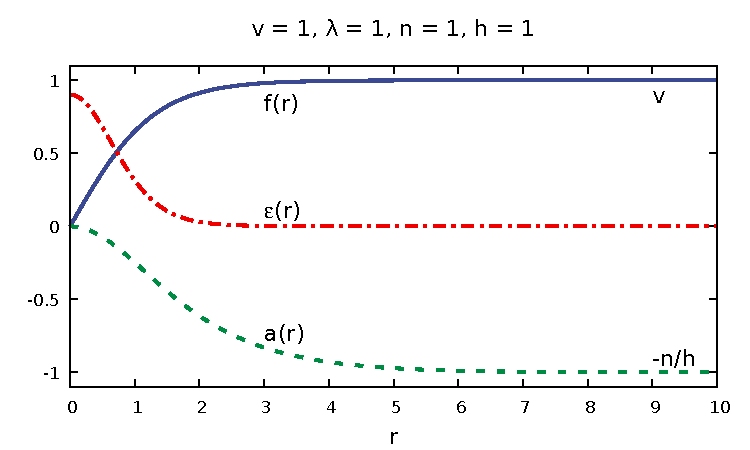
\includegraphics[scale=1]{./figures/local_str.pdf}
	\caption{Local string profile, for the scalar field $\phi$ and $a$ and the energy density $\varepsilon$, as a function of the distance from the core $r$.}
	\label{fig:local_str}
\end{figure}

\section{The mass of a local U$(1)$ string}
By simple arguments, we can estimate the order of magnitude of the mass of a local U$(1)$ cosmic string. The only quantity with dimension is the vacuum expectation value $v$ which has dimension of energy. The tension of the string $\mu$ has dimensions of force, that is, energy squared, therefore
\begin{equation}
	\mu \propto v^2.
\end{equation} 
In order to find the proportionality constant we first perform the following substitution of  $\phi$, $A^{\mu}$ and $x^{\mu}$ to dimensionless variables
\begin{eqnarray*}
	\phi & = & v\tilde \phi \\
	A^{\mu} & = & v\tilde A^{\mu}    \\
	x^{\mu} & = & \frac{1}{hv}\tilde x^{\mu} .
\end{eqnarray*}
This way, the tension of the string reads
\begin{equation}
	\mu = 2\pi v^2 \int_0^{\infty} \tilde rd\tilde r \, \left(\frac{1}{2}\left( D^{\tilde\mu} \tilde\phi\right)^{*} D_{\tilde\mu} \tilde\phi +\frac{1}{4} \tilde{F}^{\tilde\mu\tilde\nu}\tilde{F}_{\tilde\mu\tilde\nu} +\frac{\beta}{8}(1- \tilde{\phi}^*\tilde{\phi})^2\right),
\end{equation}
where the tildes in the indices indicate derivatives with respect to $\tilde x^{\mu}$ and $\beta = \frac{2\lambda}{h}$. According to Ref.\ \cite{bogo1975} the integral for $\beta = 1$ and $n=1$ is 1/2. In this case the tension of the string reads 
\begin{equation}
	\mu = \pi v^2.
\end{equation}

We expect at least one cosmic string per horizon volume. The length of an horizon is $\sim H^{-1}_0$, where $H_0$ is Hubble's constant today. So, a cosmic string can have a length of at least 
\begin{equation}
H^{-1}_0 \sim   10^{10}\ \text{years} \left(\frac{1\ \text{pc}}{3.26\ \text{years}}\right) \sim 10^{10}\ \text{pc}.
\end{equation}
%\begin{eqnarray}
%H_0^{-1} & \sim & 10^{10}\ \text{years} \left( \frac{3\times 10^7 \text{ s}}{1 \text{ year}}\right)\left( \frac{1}{6.58\times 10^{-25} \ \text{GeV} \ \text{s}}\right)  \sim 10^{42} \ \text{GeV}^{-1} \nonumber\\
% & \sim  & 10^{10}\ \text{years} \left(\frac{1\ \text{pc}}{3.26\ \text{years}}\right) \sim 3\times 10^{9}\ \text{pc}.
%\end{eqnarray}
The tension is of the order of
\begin{equation}
	v^2 = v^2 \left(\frac{10^{15}}{0.2\ \text{GeV m}}\right)\left(\frac{10^{-27}\ \text{kg}}{1\ \text{GeV}}\right)\left(\frac{3\times 10^{16} \ \text{m}}{1\ \text{pc}}\right) \sim 10^5 \left(\frac{v}{1 \ \text{GeV}}\right)^2 \ \frac{\text{kg}}{\text{pc}}.
\end{equation}
The mass of a cosmic string, related to a local symmetry, is therefore of the order of
\begin{equation}
M_{\text{string}} \sim v^2H_0^{-1} \sim 10^5 \left(\frac{v}{1\ \text{GeV}}\right)^2\  \frac{\text{kg}}{\text{pc}}\ 10^{10}\ \text{pc} \sim 10^{15} \left(\frac{v}{1 \ \text{GeV}}\right)^2 \ \text{kg}. 
\end{equation}
If we insert $v = 246 \ \text{GeV}$, then the string would have a mass of $\sim 10^{19}\ \text{kg}$. This is four orders of magnitude smaller than the mass of the Moon $\sim 10^{23} \ \text{kg}$, or eleven orders of magnitude times smaller than the mass of the Sun $\sim 10^{30} \ \text{kg}$. Because of its shape and small tension (compared to cosmic strings originated from a GUT), gravitational detection of a electroweak cosmic string would be difficult.


%By simple arguments, we can estimate the order of magnitude of the mass of a local U$(1)$ cosmic string. First, we compute the energy density of the gauge field
%\begin{equation}
%	\varepsilon(A_{\mu}) = \frac{1}{4}F_{\mu\nu}F^{\mu\nu}  = \frac{1}{2}\left(\nabla\times \vec{A}\,\right)^2 = \frac{1}{2}\left(\frac{\partial_r a}{r}\right)^2.
%\end{equation}
%	Near the string core, we can estimate the derivative to be $\partial_r a \sim \frac{-n/h}{l_A}$, where $l_A = 1/m_A$ is the Compton length and $m_A = hv$ the mass of the gauge boson after SSB. Therefore, near the core, the energy density of the string is
%	\begin{equation}
%		\varepsilon(A_{\mu}) =\frac{1}{4} F_{\mu\nu}F_{\mu\nu} \approx\frac{1}{2} \left(\frac{n}{hl^2_A}\right)^2,
%	\end{equation}
%and the energy per unit length is
%\begin{equation}
%		\frac{E}{z}(A_{\mu}) \approx \frac{1}{2} \left(\frac{n}{hl^2_A}\right)^2l_A^2 = \frac{1}{2}n^2v^2.
%	\end{equation}
%The scalar field contribution to the energy density is	
%\begin{equation}
%	\varepsilon(\phi)=\frac{1}{2}(D_i\phi)^*(D_i\phi) + \frac{m^2}{2}\phi^*\phi + \frac{\lambda}{4}(\phi^*\phi)^2 +\frac{\lambda}{4}v^4.
%\end{equation}
%Near the string core, $\phi\sim 0$ and $\partial_r \phi \sim v/l_{\phi}$, where $l_{\phi}$ is the Compton length of the scalar field with $l_{\phi} = 1/m_{\phi}$ and $m_{\phi} = \sqrt{2\lambda} v$. Therefore, the energy density due to the scalar field is approximately
%\begin{equation}
%	\varepsilon(\phi)\approx\frac{1}{2}\left(\frac{v}{l_{\phi}}\right)^2 + \frac{1}{4}\lambda v^4,
%\end{equation}
%and the energy per unit length 
%\begin{equation}
%	\frac{E}{z}(\phi) \approx \frac{1}{2}\left(\frac{v}{l_{\phi}}\right)^2l_{\phi}^2 + \frac{1}{4}\lambda v^4l_{\phi}^2 =  \frac{5}{8}v^2.
%\end{equation}
%Hence, the contribution to the tension due to the fields is approximately
%\begin{equation}
%	\frac{E}{z} \approx  \left(\frac{1}{2}n^2 + \frac{5}{8}\right)v^2.
%\end{equation}
%If $\left(\frac{1}{2}n^2 + \frac{5}{8}\right)\sim\text{O}(1)$, the energy per unit length is of the order of $v^2$. 
%We expect at least one cosmic string per horizon volume. The length of an horizon is $\sim H^{-1}_0$, where $H_0$ is Hubble's constant today. So, a cosmic string can have a length of at least 
%\begin{equation*}
%H_0^{-1} \sim 10^{10}\ \text{years} \left( \frac{3\times 10^7 \text{ s}}{1 \text{ year}}\right)\left( \frac{1}{6.58\times 10^{-25} \ \text{GeV} \ \text{s}}\right)  \sim 10^{42} \ \text{GeV}^{-1}.
%\end{equation*}
%The mass of a cosmic string, related to a local symmetry, is therefore of the order of
%\begin{equation}
%M_{\text{string}} \sim v^2H_0^{-1} \sim v^2 10^{42}\ \text{GeV}^{-1}\left(\frac{10^{-27}\ \text{kg}}{1 \ \text{GeV}} \right) \sim 10^{15} v^2 \left[ \frac{\text{kg}}{\text{GeV}^{-2}}\right]. 
%\end{equation}
%If we insert $v = 246 \ \text{GeV}$, then the string would have a mass of $\sim 10^{19}\ \text{kg}$. This is eleven orders of magnitude times smaller than the mass of the sun $\sim 10^{30} \ \text{kg}$, so the gravitational detection of such a single string is not realistic.

\section{The search for cosmic strings}
There exist several ways of searching for cosmic strings, such as their con\-tri\-bu\-tions to the CMB power spectrum, gravitational lensing, their emission of grav\-i\-ta\-tion\-al radiation, emission of particles, etc. We discuss briefly some of the most popular ways of trying to detect cosmic strings. We refer to a very useful dimensionless quantity 
\begin{equation}
	G\mu,
\end{equation} 
where $G = \frac{1}{(1.2\times 10^{19} \ \text{GeV})^2} $ is Newton's gravitational constant and $\mu$ is the tension of the string. It measures, for instance, the gravitational coupling of the string.

\subsection{CMB power spectrum measurements}
In the early universe, a short time after the \textit{Big Bang}, photons were coupled to matter forming a hot plasma of baryons, leptons and photons. At this stage, photons were not able to travel long distances. Approximately when the universe was $300,000$ years young, the first atoms were formed. Since atoms are neutral, photons decoupled from matter, a process known as recombination. After that, photons were able to travel long distances without being absorbed by a particle. This radiation is known as the Cosmic Mi\-cro\-wave Background (CMB), and permeates the entire universe. The CMB follows almost perfectly a thermal spectrum of black body radiation at a temperature of $2.73\ \text{K}$. However, the thermal spectrum has temperature fluctuations or anisotropies.

Several missions such as COBE, WMAP and PLANCK were design to measure the CMB photons energy anisotropies. In Figure \ref{fig:cmb} we see the CMB temperature distribution as captured by PLANCK. When several regions of the CMB map are analyzed at different angular scales, we can observe how the temperature fluctuations behave and we can plot its power spectrum, see Figure \ref{fig:powerspec}.

If cosmic strings exist, they would have a distinct footprint in the CMB power spectrum.  In particular, photons passing near a cosmic string would have a redshift which results in step-like discontinuities in the CMB. Ac\-cord\-ing to Ref.\ \cite{kaiser1984}, the discontinuities in the CMB temperature deviation due to cosmic strings is of the order of
\begin{equation}
	\frac{\Delta T}{T} = 8\pi G \mu \beta,
\end{equation}
where $\beta$ is the transverse velocity of the string and $T$ is the temperature and $\Delta T$ is the temperature fluctuations.
In fact, measurements of the CMB anisotropies can set constraints to the tension of cosmic strings. The con\-straint to the tension according to Ref.\ \cite{Lazanu_2015}, using PLANCK's data, is
\begin{equation}
	G\mu \lesssim 1.49\times 10^{-7}.
\end{equation}
The excitement of cosmic strings in the early 80s, was that they could have explained the formation of large structures \cite{kibble1986}. However, for cosmic strings to have an important impact for the formation of structures we need that $G\mu\sim 10^{-6}$. This would have a great impact in the power spectrum: the acoustic peaks at angle scales less than $1^{\circ}$ would be smoothen out, but this is not the case. That cosmic strings cannot explain the acoustic peaks in the CMB power spectrum does not mean that they are rule out. But this constrains the contribution of cosmic strings and other topological defects to the CMB power spectrum. The observations indicate that the contribution of topological defects to the CMB cannot be more than $10\%$ \cite{pogo2006}.

\begin{figure}
	\centering
	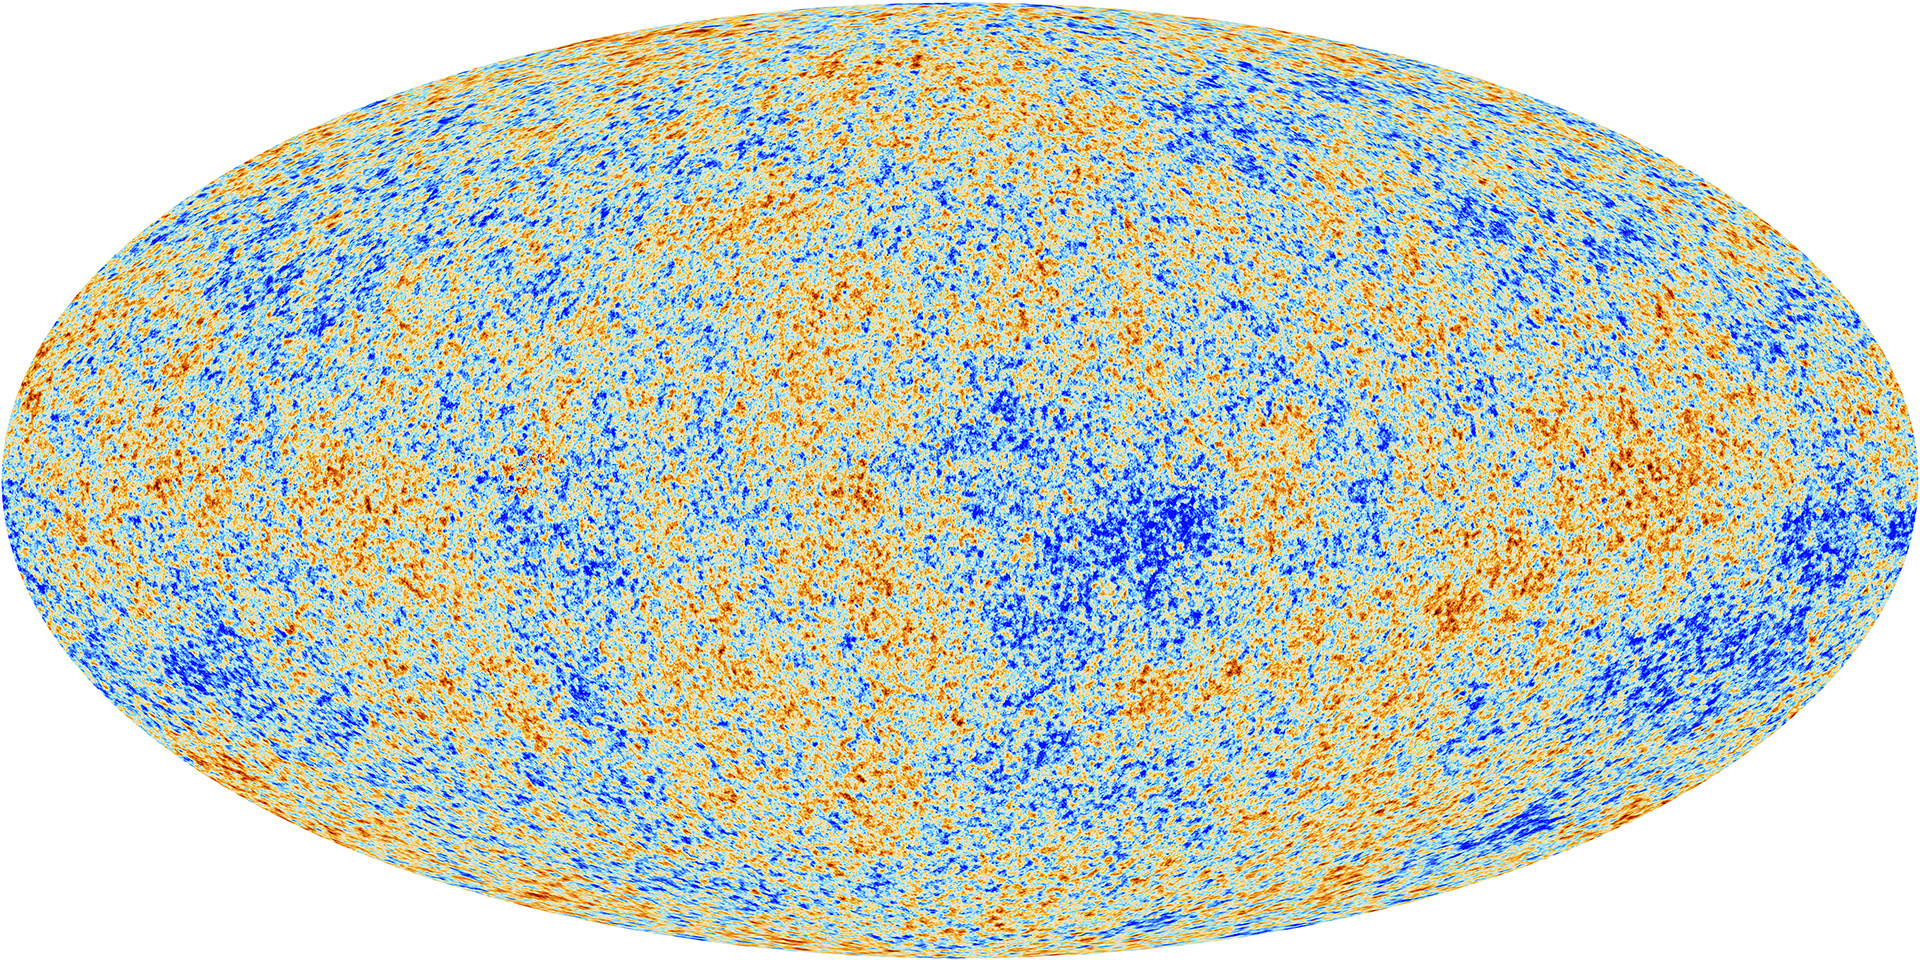
\includegraphics[scale=0.2]{./figures/Planck_CMB.jpg}
	\caption{CMB as captured by PLANCK. Figure taken from Ref.\ \cite{cmb}.}
	\label{fig:cmb}
\end{figure}


\begin{figure}
	\centering
	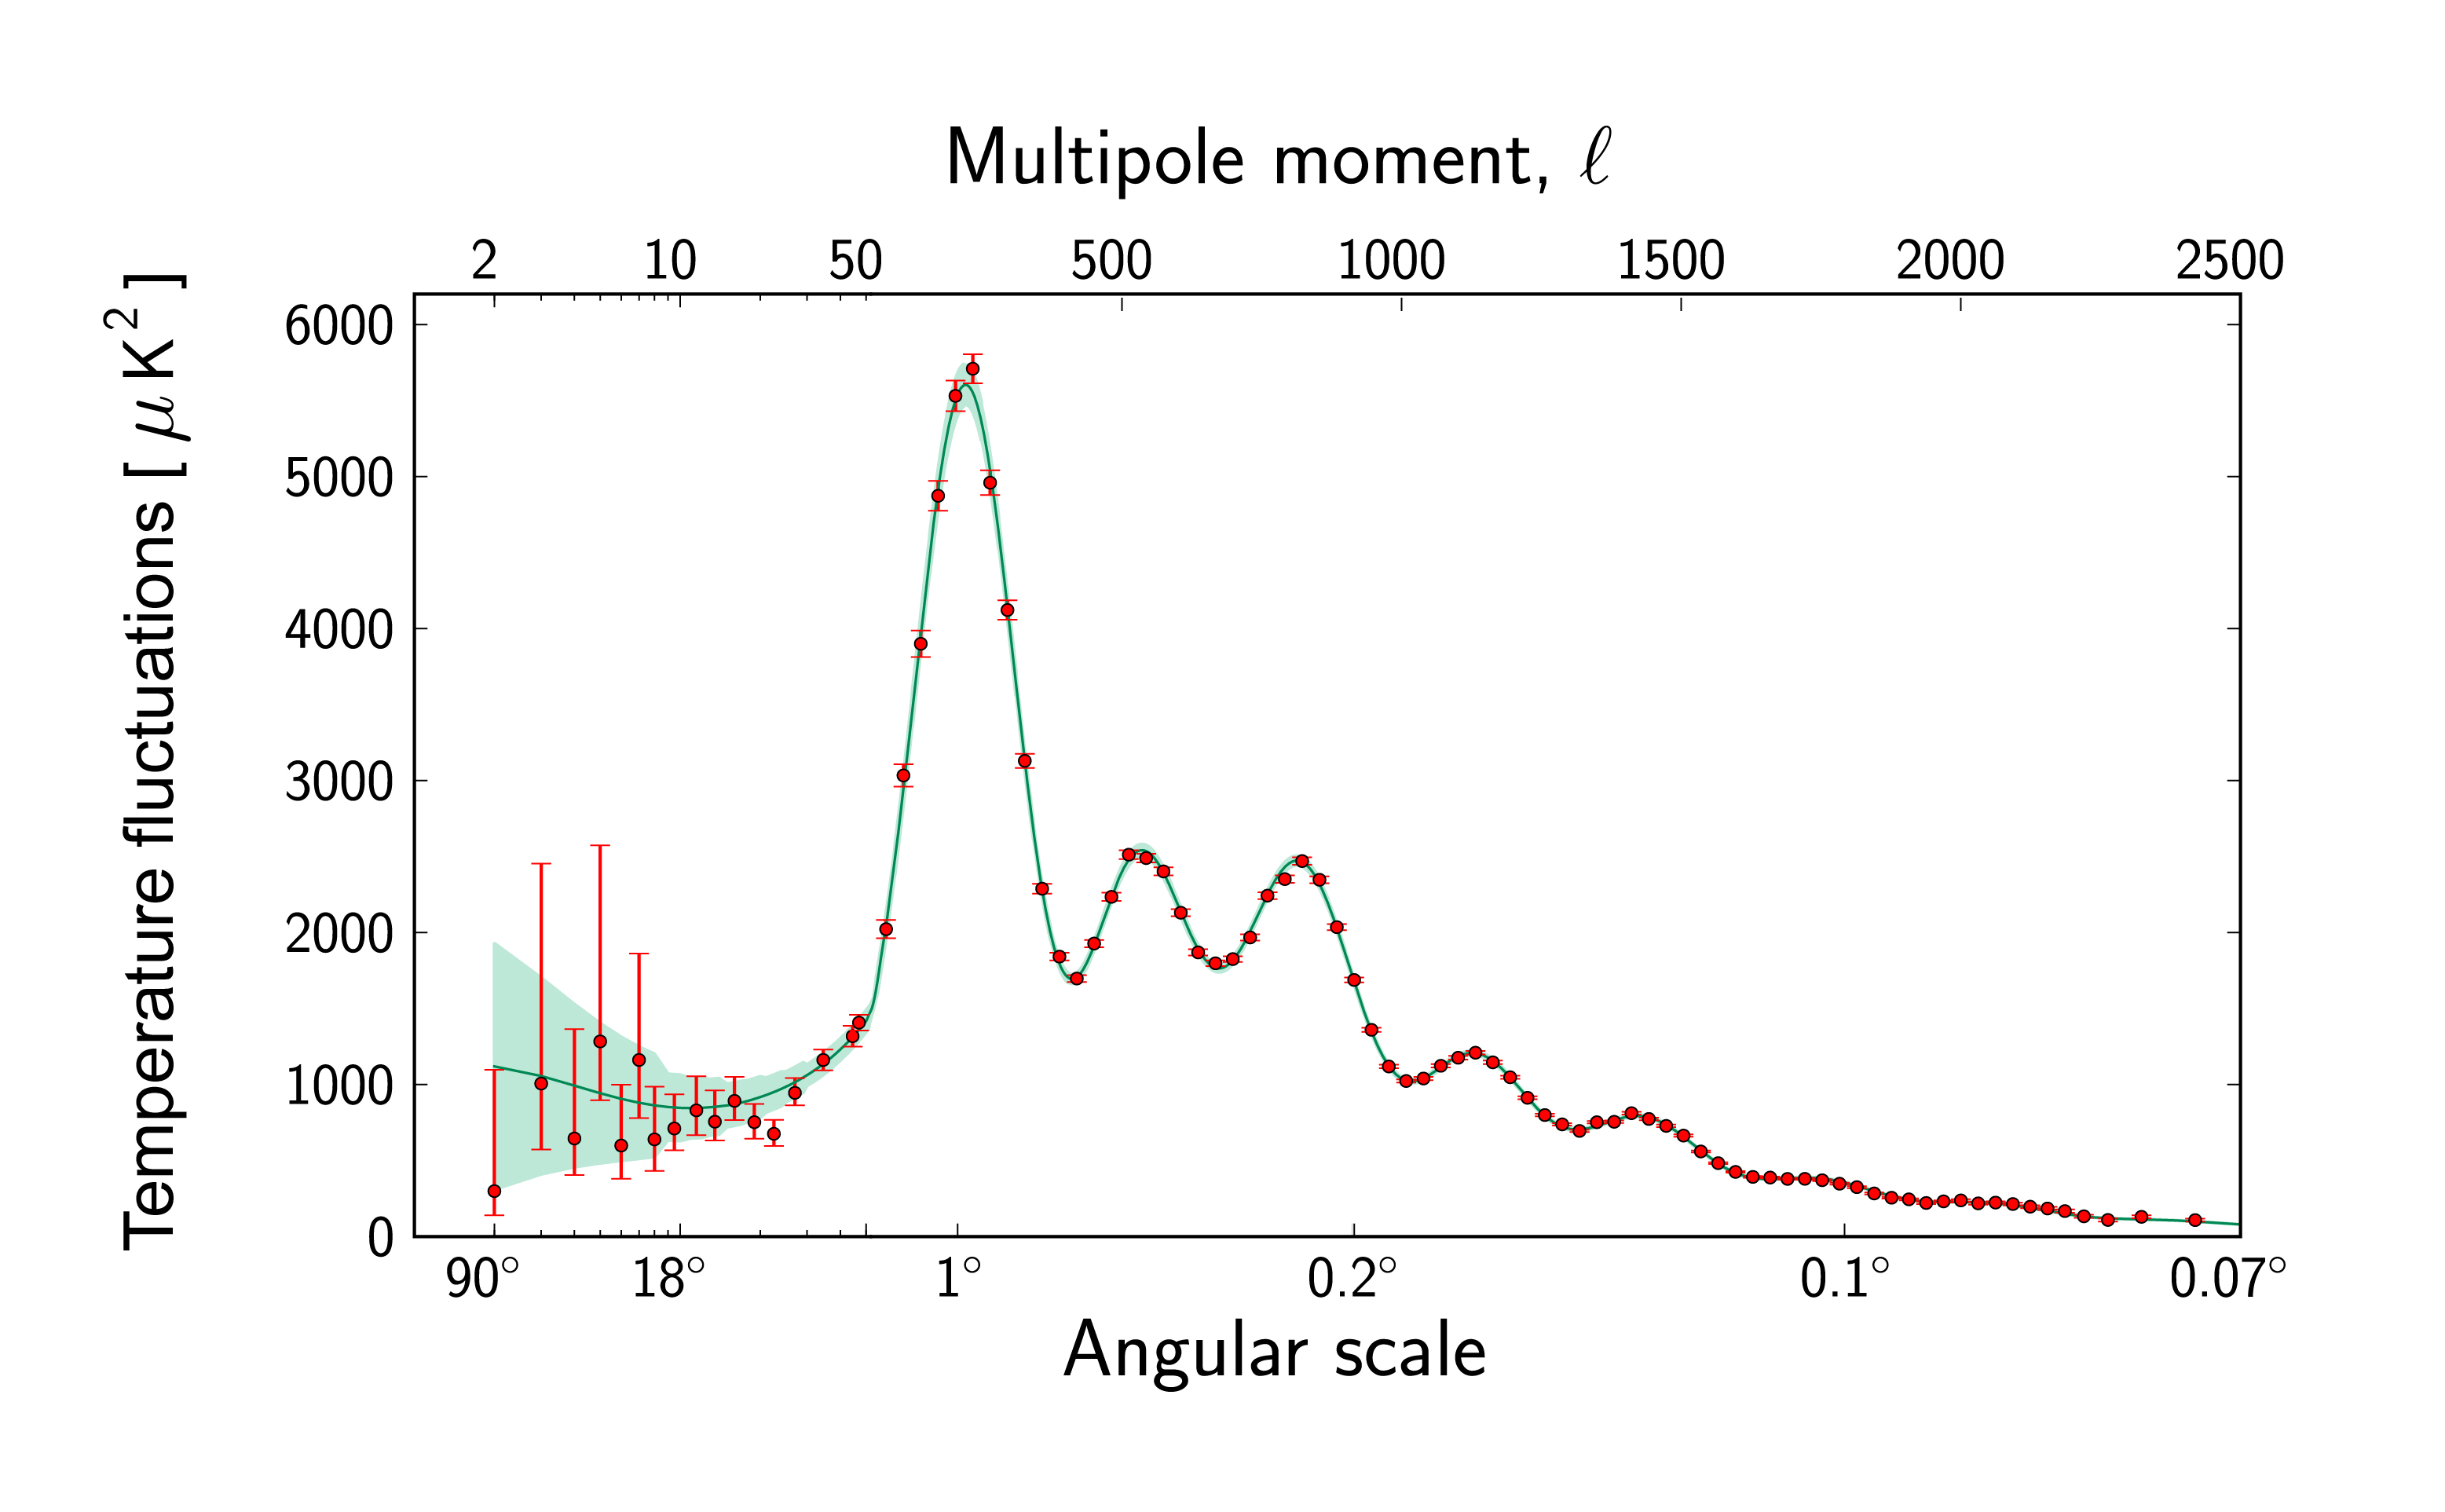
\includegraphics[scale=0.5]{./figures/Planck_Power_Spectrum.jpg}
	\caption{Cosmic Microwave Background power spectrum. Cosmic strings as a seed for large structures is now ruled out, since they do not explain the acoustic peaks at angular scales less than $1^{\circ}$. Plot taken from \cite{powerspec}.}
	\label{fig:powerspec}
\end{figure}



\subsection{Gravitational lensing}
Let us consider a static string along the $z$-axis. In the zero width limit its energy-momentum tensor reads
\begin{equation}
	T^{\mu\nu} = \mu\delta(x)\delta(y)\,\text{diag}(1,0,0,-1).
	\label{eq:energytensor}
\end{equation}
The metric tensor far outside a cosmic string is known to be locally flat, it reads
\begin{equation}
	ds^2 = dt^2-dr'^2-r'^2d\varphi'^2-dz^2,
	\label{eq:metric}
\end{equation}
where $r'$ and $\varphi'$ are defined through the relations 
\begin{equation}
(1-8G\mu\log(r/r_0))r^2 = (1-8G\mu)r^2, \ \ \ \varphi' = (1-4G\mu)\varphi.
\end{equation}
Here $r\in [0,\infty] $ and $\varphi\in[0,2\pi)$ are the usual variables in cylindrical co\-or\-di\-nates and $r_0$ is a constant. This implies that there is an \textit{angular deficit}, which is defined as 
\begin{equation}
\Delta \varphi = \varphi_{\text{max}} - \varphi'_{\text{max}} = 2\pi -2\pi(1-4G\mu) = 8\pi G\mu.
\end{equation}
Physically, it means that a light source, such as a galaxy or a star, behind the core of a string produces a double image separated by the angle 
\begin{equation}
	\alpha = \frac{l_1}{l_2}\Delta\varphi\sin\theta,
\end{equation}
assuming $G\mu\ll 1$, where $l_1$ is the distance between the string and the observer, $l_2$ is the distance between the string and the object and $\theta$ is the angle that the string makes with the plane of the observer and and the object, see Figure \ref{fig:lens}. That is, a non-zero angular deficit suggests that a cosmic string would act as a gravitational lens.

\begin{figure}
	\centering
	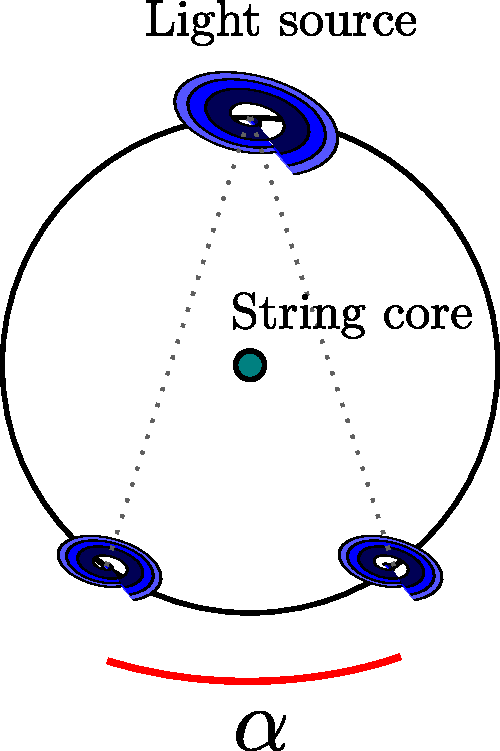
\includegraphics[scale=0.75]{./figures/lens.pdf}
	\caption{Gravitational lensing by a massive cosmic string. An object is behind the string core. The telescopes on Earth would observe two similar close objects separated by the angle $\alpha$.}
	\label{fig:lens}
\end{figure}

For example, we consider an energy scale of $v\sim 10^{16}\ \text{GeV}$, then $G\mu\sim 10^{-6}$, typical of a Grand Unified Theory. A cosmic string, such as one formed due to the spontaneous symmetry breaking of a GUT gauge group, would be very massive and would have a dramatic effect on the lensing of objects behind it. The angular defect of such a string would be $\Delta\varphi = 8\pi G\mu \simeq 5.18''$ \cite{Vilenkin1994}.

 In principle,  an observational way to detect a cosmic string would be to look for a line of double objects. If this is observed, we could conclude that it was caused by a very massive object such as a cosmic string. In Figure \ref{fig:numlens} we see three examples of how a gravitational lens produced by a massive cosmic string would look like, taken from Ref.\ \cite{stringlens}.

\begin{figure}
	\centering
	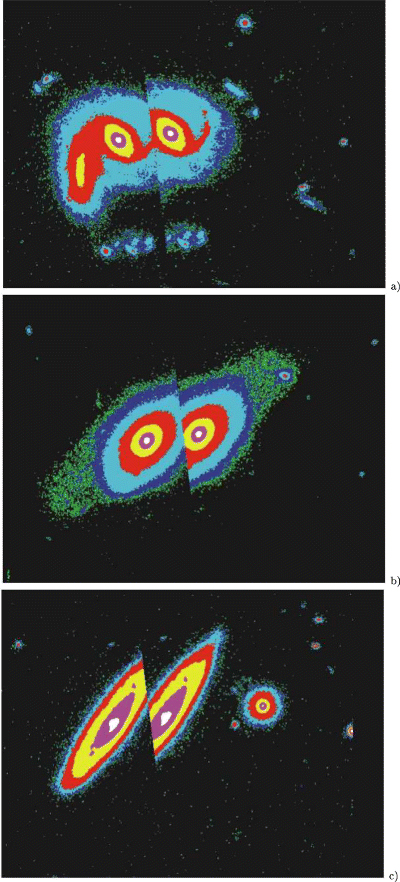
\includegraphics[scale=0.5]{./figures/stringlensing.jpeg}
	\caption{Gravitational lensing by a massive cosmic string generated by numerical simulations, illustration taken from Ref.\ \cite{stringlens}.}
	\label{fig:numlens}
\end{figure} 

In 2003, two close galaxies called CSL-1, see Figure \ref{fig:csl1}, were thought to be two copies of the same galaxy. That is, a gravitational lens produced by a cosmic string, Ref.\ \cite{Sazhin2003}. However, it was ruled out in 2006 by careful measurements on the brightness of the galaxies, see Ref.\ \cite{Agol2006}.

\begin{figure}
	\centering
	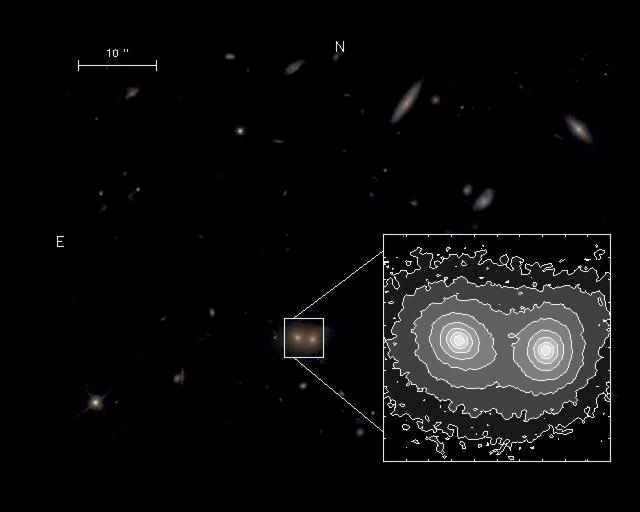
\includegraphics[scale=0.5]{./figures/csl1.jpg}
	\caption{CLS-1 candidate for two copies of the same galaxy as a result of the gravitational lensing of a cosmic string, illustration taken from \cite{Agol2006}.}
	\label{fig:csl1}
\end{figure}
 
 
  Besides gravitational lensing, another gravitational observation would be the detection of gravitational waves.
 
\subsection{Gravitational waves} 

Since the first detection of gravitational waves \cite{PhysRevLett.116.061102}, one of the most realistic way of possible detection of cosmic string is by their emission of gravitational radiation.
According to General Relativity, an oscillating cosmic string loop loose energy by emitting gravitational waves with a power of
\begin{equation}
	P = \Gamma G\mu^2,
\end{equation}
where $\Gamma$ is a constant. 

The production of cosmic string loops can be of various ways, see Figure \ref{fig:loops}. When two strings collide, or when a single string backs on itself, they could form either two new strings, or a new string and a loop. In fact, oscillating loops have a characteristic emission of gravitational radiation produced by \textit{kinks} and \textit{cusps}, through interactions with other strings or with itself. \textit{Kinks} are discontinuities in their worldsheet $x^{\mu}$ or $\dot{x}^{\mu}$. \textit{Cusps} are pointy regions on the string, see Figure \ref{fig:cusp}. A cusp in a loop is formed by two modes, one traveling to the left and the other to the right at the speed of light. Cusps in a loop are short lived and produce a particular signal of gravitational waves beamed in the direction of the cusp. On the other hand, kinks travel along the string and produce a beam of gravitational waves in a fan-like manner.

The Virgo/LIGO Collaboration put constraints on the tension of cosmic strings \cite{PhysRevLett.126.241102}: it found that, referring to loop radiation, the constraint for the tension is
\begin{equation}
	G\mu \lesssim 4\times10^{-15}.
\end{equation}
Unfortunately, this collaboration did not find any evidence of gravitational waves produced by cosmic strings.

\begin{figure}
	\centering
	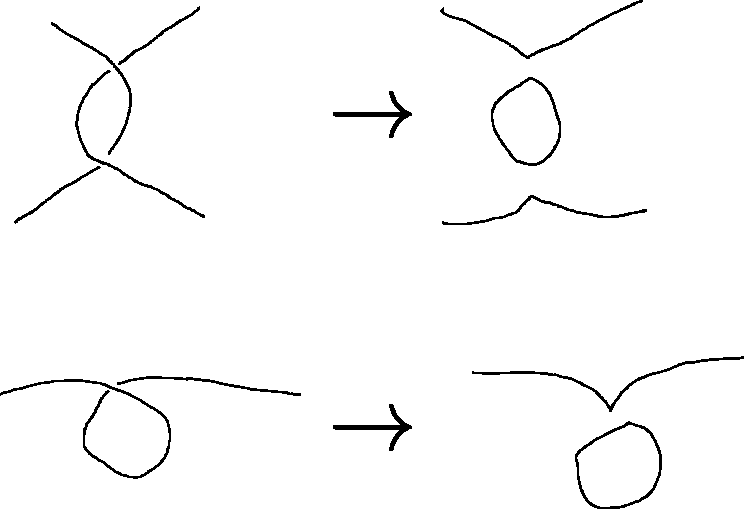
\includegraphics[scale=1]{./figures/kinks.pdf}
	\caption{Formation of loops. Above: two strings intersect and form two new strings and a loop. Below: A string intersects with itself leaving a new string and  a loop. However, the interaction of strings will not always produce loops.}
		\label{fig:loops}
\end{figure}


\begin{figure}
	\centering
	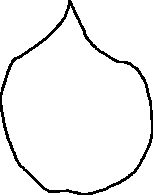
\includegraphics[scale=1.5]{./figures/cusp.pdf}
	\caption{A loop with a cusp. Near the cusp the speeds of the right and left modes are the speed of light.}
		\label{fig:cusp}
\end{figure}